
\chapter{Metodologia}

Para a execução deste projeto, optou-se pelo uso de componentes amplamente disponíveis no mercado a relativamente baixo
custo, bem como software disponível gratuitamente no site do fabricante. Essas escolhas visam facilitar a
reproducibilidade do projeto, bem como tornar o resultado final do projeto mais eficiente, produzindo o resultado
desejado com o menor custo. 

Um outro fator relevante que impactou a escolha dos componentes a serem utilizados no projeto é a compatibilidade entre
eles - seja ela mecânica, eletrônica ou mesmo de software. Diferentemente de uma solução completa oferecida por
um só fabricante, em que há garantia de operação harmoniosa entre os componentes, este trabalho envolveu a composição de
diferentes partes, pelo que se tornou necessário avaliar a viabilidade de se utilizar todas elas em conjunto.

Ainda assim, dada a necessidade de se utilizar peças com formatos e dimensões específicas para a aplicação em questão,
optou-se também pelo uso de técnicas de impressão 3D. Essa decisão é compatível com o objetivo geral de baixos custos, e
também resolve problemas relacionados à montagem mecânica.


\section{Hardware}
A aquisição dos componentes de hardware empregados neste projeto se deu, em boa parte, por meio de lojas importadoras de
componentes. Optou-se por componentes de baixo custo e, ao mesmo tempo, comumente utilizados em projetos dessa natureza,
a fim de se ter amplo apoio da comunidade na resolução de eventuais problemas encontrados no desenvolvimento da solução.
A tabela \ref{custos} apresenta os custos de cada componente de hardware adquirido para uso exclusivo neste projeto
(excluindo, portanto, equipamentos empregados mas não utilizados apenas nele, como a impressora 3D).


\begin{quadro}[htb]
	\caption{Lista de componentes, materiais e seus custos - valores em reais (R\$) \label{custos}}
	 \begin{tabular}{|c|c|c|c|}
		\hline
		\textbf{Componente ou Material} & \textbf{Valor unitário} & \textbf{Quant} & \textbf{Valor Total} \\ \hline
		Driver Ponte H L298N \cite{l298n_produto} &  22,90 & 3 &  68,70   \\ \hline
		Motor DC 6V 210 RPM \cite{motor_dc_6v_produto} &  90,00 & 3 &  270,00   \\ \hline
		Filamento PLA \cite{filamento_pla_produto} &  99,99 & 1 &  99,99   \\ \hline
		Kit 4 rodas Omnidirecional \cite{omin_wheel_produto} &  131,35 & 1 &  131,35   \\ \hline
		Kit 4 peças eixo roda \cite{omin_wheel_produto} &  42,15 & 1 &  42,15   \\ \hline
		STM32 (microcontrolador) \cite{stm32_produto} &  46,90 & 1 &  46,90   \\ \hline
		Bateria selada 6V \cite{bateria_6v_produto} &  69,90 & 1 &  69,90  \\ \hline
		Powerbank &  119,90 & 1 &  119,90   \\ \hline
		Paquímetro  &  49,90 & 1 &  49,90   \\ \hline
		Ferro de solda &  43,20 & 1 &  43,20   \\ \hline
		Solda &  12,99 & 1 &  12,99   \\ \hline
		Conector mjjst macho &  4,90 & 3 &  14,70   \\ \hline
		Conector mjjst femea &  4,90 & 3 &  14,70   \\ \hline
		Garra jacaré &  1,65 & 2 &  3,30   \\ \hline
		Driver Ponte H DTV8833 \cite{drv8833_produto} &  15,00 & 3 &  45,00   \\ \hline
		Módulo Bluetooth \cite{hc05_produto} &  35,00 & 1 &  35,00   \\ \hline
		Mini Protoboard &  5,00 & 2 &  10,00   \\ \hline
		Protoboard 830 &  16,00 & 1 &  16,00   \\ \hline
		Jumper macho-macho &  8,00 & 1 &  8,00   \\ \hline
		Pasta de solda &  14,99 & 1 &  14,99   \\ \hline
		Sugador de solda &  12,99 & 1 &  12,99   \\ \hline	
		\textbf{CUSTO TOTAL} & & & \textbf{ 1.129,66}   \\ \hline
	\end{tabular}
\end{quadro}

\subsection{Componentes eletrônicos}

\subsubsection{Motor DC e encoder}
Para a versão inicial do robô, foi decidido trabalhar com motor DC.
Motores DC são mais difíceis de controlar que motores de passo, porém tem uma resposta mais rápida, e se o controle for
bem aplicado, podem ter também um melhor desempenho. A complexidade do controle de um motor DC apresenta um bom desafio
para aplicação dos conceitos e disciplinas do curso de Engenharia de Instrumental, Automação e Robótica. O motor DC 
escolhido foi um de 6V 210rpm, com taxa de redução de 1:34. Tal motor já possui um encoder magnético acoplado, com 11
PPR (\textit{"Pulses Per Revolution"}), resultando em um encoder com resolução de 374 PPR.

\begin{figure}[htb]
	\centering
	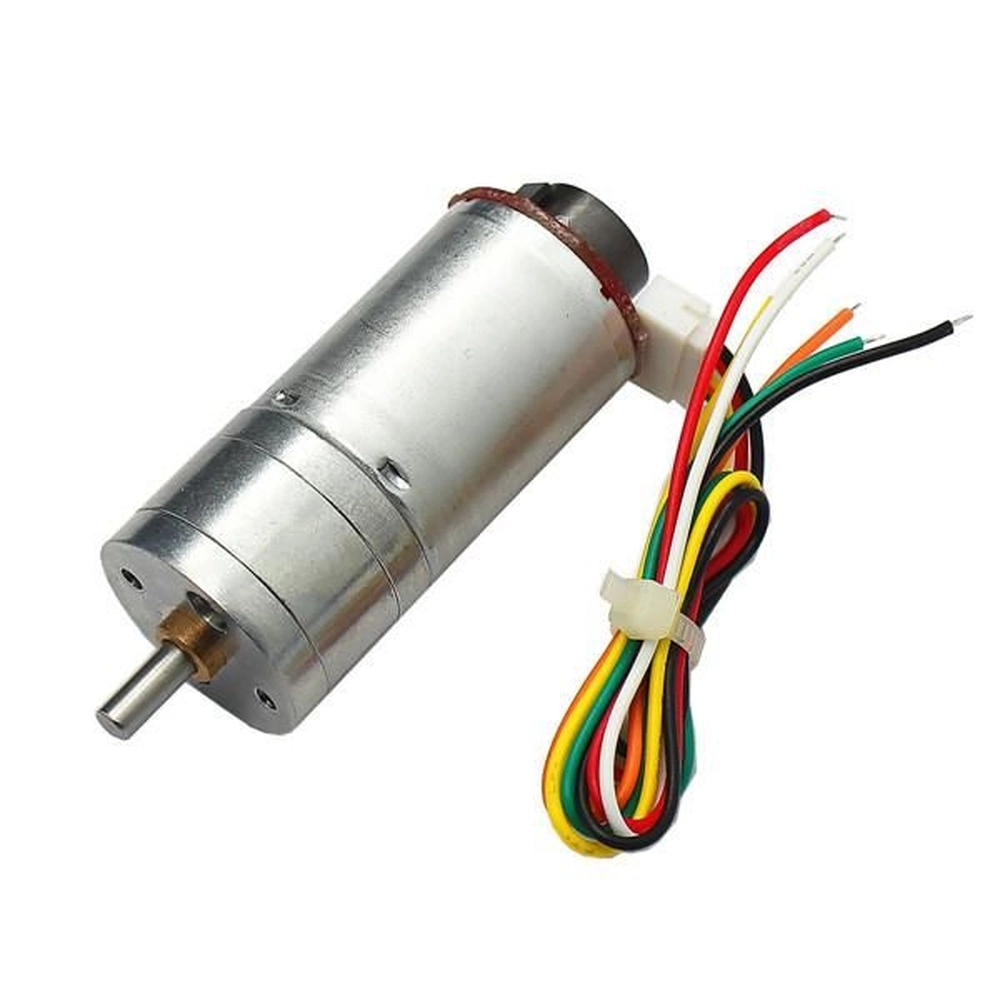
\includegraphics[width=0.7\textwidth]{figures/CHR_GM25_370}
	\caption{Motor DC 6V \cite{motor_dc_6v_encoder}}
\end{figure}

\begin{quadro}[htb]
\caption{\label{Especificacoes_motordc_6v}Especificações do motor DC 6V}
	 \begin{tabular}{|c|c|c|c|}
		\hline
		\textbf{Especificação} & \textbf{Valor} \\ \hline
		Tensão nominal & DC 6V  \\ \hline
		Velocidade sem carga  & 210RPM 0.13A  \\ \hline
		Eficiência máxima & 2,0kg.cm/170rpm/2,0W/0,60A   \\ \hline
		Poder máximo & 5,2kg.cm/110rpm/3,1W/1,10A   \\ \hline
		Torque de parada  & 10kg.cm 3.2A    \\ \hline
		Taxa de Redução do Retardador & 1:34  \\ \hline
		Resolução do salão & Razão Hall x 34,02 = 341,2PPR  \\ \hline
	\end{tabular}
	\fonte{\cite{chinhai_motor}}
\end{quadro}


\subsubsection{Driver de Motor}
Nas etapas iniciais do projeto, testou-se driver Ponte H L298N para ligar cada motor. Esse driver suporta até 2A em
operação DC \cite{datasheel_l298n}. A corrente de operação máxima do motor é de 1.1A; contudo, a corrente de parada
pode chegar a 3.2A. Além disso, o L298N também causa uma queda de tensão significativa: a uma corrente de 1A, a queda
observada chegou a até 3.2V, fazendo com que o motor não receba a tensão necessária para operar nas condições
desejadas \cite{datasheel_l298n}. As observações são compatíveis com as expectativas de faixa de operação do L298N - a
seu uso é recomendado para tensões entre 12V a 40V, em que a queda de tensão observada não seja tão significativa
relativamente. Devido à natureza da aplicação deste projeto, com o motor de 6v, a queda de tensão acaba sendo
intolerável, inviabilizando assim o uso da ponte H L298N.

Após essas considerações e observações, optou-se por um driver apropriado para uso em baixas tensões, o DRV8833
\cite{datasheel_dvr8833}.


\begin{figure}[htb]
	\centering
	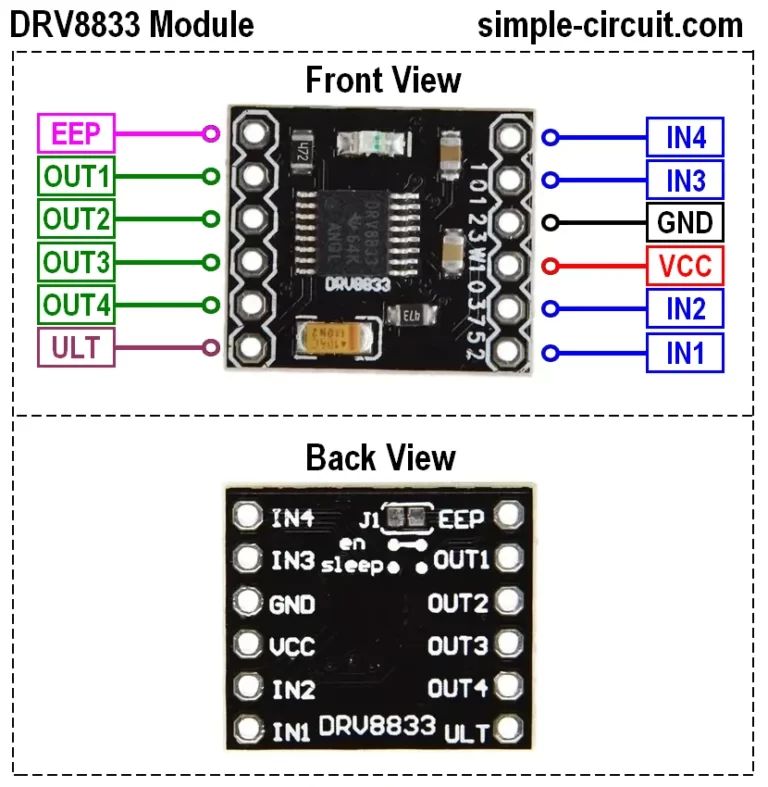
\includegraphics[width=0.5\textwidth]{figures/DRV8833-Dual-Driver-Pinout}
	\caption{Driver Ponte H DVR8833 \cite{DRV8833_image}}
\end{figure}

\subsubsection{Microcontrolador}

Como opção de microcontrolador, optou-se pelo uso do STM32F103C8 (abreviado como STM32 ao longo deste trabalho),
também conhecido como Blue Pill. Possui como processador o ARM Cortex-M3, e tem 64Kbs de memória flash.  Possui também 7 timers, 2 ADCs, e 9 interfaces de comunicação, incluindo I2C (\textit{Inter-Integrated Circuit}), USART 
\textit{Universal Synchronous Asynchronous Receiver Transmitter}), SPI (\textit{Serial Peripheral Interface}), CAN e
USB 2.0. O STM32 apresenta 7 pinos que suportam canais de PWM de 5V, e outros 8 canais de 3.3V, e pode ser alimentado
via microUSB de 5V. Existem 3 grupos de pinos,  $P_{A}$,  $P_{B}$ e  $P_{C}$: os pinos PA vão de $P_{A0}$ 
a $P_{A15}$, PB indo de $P_{B0}$ a $P_{B15}$, e PC com apenas 3 pinos, $P_{C13}$, $P_{C14}$ e $P_{C15}$.

Para carregar o projeto no microcontrolador, utilizou-se um gravador ST-LINK USB.

\begin{figure}[htb]
	\centering
	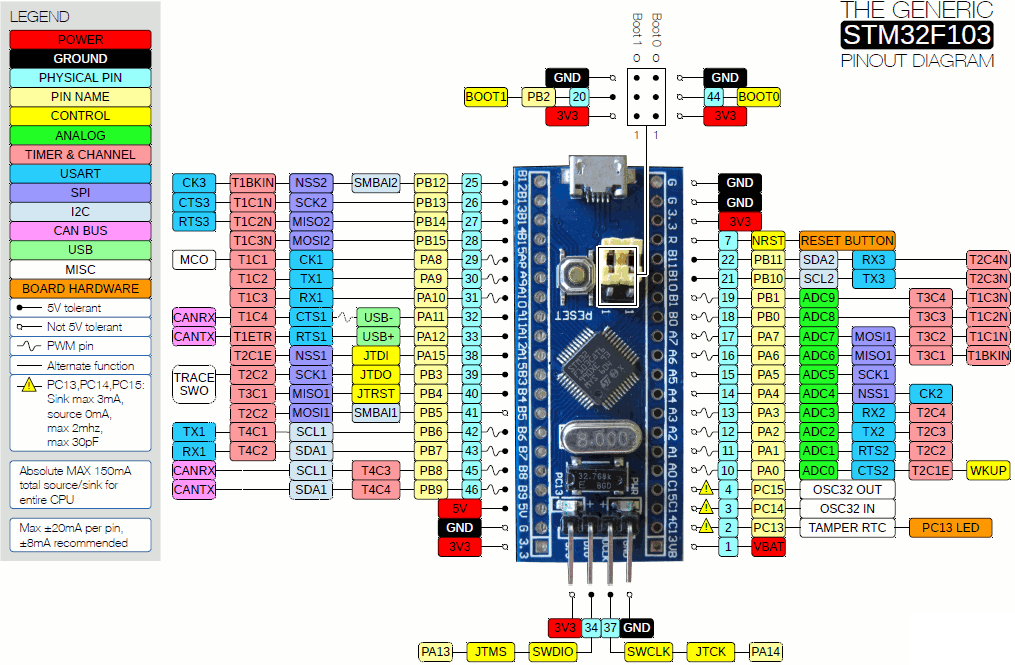
\includegraphics[width=1.0\textwidth]{figures/stm32f1_pinout}
	\caption{Diagrama de pinos do STM32F103C8}
\end{figure}

\subsubsection{Alimentação}
Para alimentar o microcontrolador, um powerbank com saída de 5V foi empregado usado, considerando que o STM32F103C8 
funciona a uma corrente abaixo de 100mA. Para alimentar os motores, durante o desenvolvimento, optou-se por uma 
bateria de chumbo-ácido de 6V 4.5Ah.

\subsubsection{Comunicação Bluetooth para controle em aplicativo Android - Módulo HC-05}
Para controle de movimento do robô, desenvolveu-se um aplicativo Android, com uso da ferramenta MIT App Inventor. O app opera enviando para o microcontrolador comandos via Bluetooth. O STM32 recebe esses commands por meio 
do módulo de Bluetooth HC-05 (figura \ref{fig:hc_05}). A comunicação entre o HC-05 e o STM32 é serial, fazendo uso 
dos pinos da USART2 do STM32, $P_{A3}$ (RX2) e $P_{A2}$ (TX2).

\begin{figure}[htb]
	\centering
	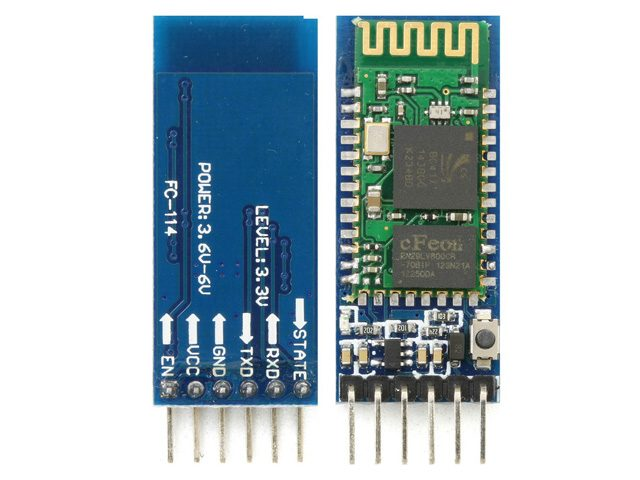
\includegraphics[width=0.5\textwidth]{figures/hc_05}
	\caption{Módulo Bluetooth HC-05}
	\label{fig:hc_05}
	\cite{hc05_image}
\end{figure}

\subsection{Fabricação e montagem}
O chassi e demais peças foram fabricados por meio de impressão 3D, usando filamento de PLA (ácido poliáctico). As
peças foram projetadas no AutoCAD, e posteriormente modeladas em 3D com o SolidWorks. A geometria do modelo
resultante de cada peça foi convertida em código G para uma impressora 3D por meio do software UltiMaker Cuda. Por
fim, a impressão das peças foi realizada em uma impressora Ender 3 S1 Pro.



% \subsection{Joystick de controle}
% Um joystick de 3 eixos para controlar o robô para testar a cinemática de movimento.
% {\color{red} É necessário aqui especificar o modelo utilizado e descrever características.}

% \subsection{Sensores}
% {\color{red} Esta subseção deve descrever os sensores utilizados e também sua finalidade.}

% \subsection{Dispositivos de comunicação}
% {\color{red} Esta subseção deve descrever os dispositivos de comunicação utilizados (Wi-fi, Bluetooth, etc) e também sua
% finalidade.}

% \subsection{Calibração de parâmetros}
% {\color{red} Caso haja necessidade de calibração de parâmetros de alguns dos componentes utilizados (sensibilidade de
% sensores, histerese de componentes mecânicos, taxa de comunicação de dispositivos, etc), os procedimentos devem ser
% descritos nesta subseção.}

\section{Software}
No desenvolvimento deste projeto, algumas ferramentas de software foram e empregadas. As principais áreas em que seu uso
se fez necessário foram na programação do STM32, no desenvolvimento do aplicativo para comunicação entre um Smartphone e
o módulo HC-05, no projeto e impressão 3D das peças da estrutura do robô, e nas simulações para obtenção empírica de
parâmetros de operação do robô.

\subsection{Programação do microcontrolador}
Nesta aplicação, o microcontrolador contém é responsável por coordenar a operação do robô. Por essa razão, foi
necessário programar tal funcionalidade em sua memória. Neste processo, foi necessário configurar os diferentes pinos de
entrada segundo suas capacidades e o uso desejado no projeto, bem como implementar o processamento dos sinais de entrada
(referentes à velocidade dos motores) e a produção de saída (valores a serem enviados como variável manipulada para os
motores do robô). É também do microcontrolador a tarefa de interpretar os comandos recebidos via Bluetooth pelo módulo 
HC-05 (e transmitidos ao STM32 via comunicação serial) e convertê-los em sinal de controle.

\subsection{Desenvolvimento de aplicativo Android}
Por meio do uso da plataforma MIT App Inventor, vou possível simplificar significativamente o desenvolvimento de um app
Android para uso neste trabalho. A plataforma fornece elementos visuais para produção da interface do app, bem como 
permite implementação de algumas funcionalidades mais comuns (como acesso à comunicação Bluetooth de um Smartphone) a 
serem associadas com esses elementos visual. A app desenvolvido tem por objetivo enviar comandos simples, relacionados
a direções a serem seguidas pelo robô, como demonstra figura \ref{fig:mit_app_inventor}.

\begin{figure}[htb]
	\centering
	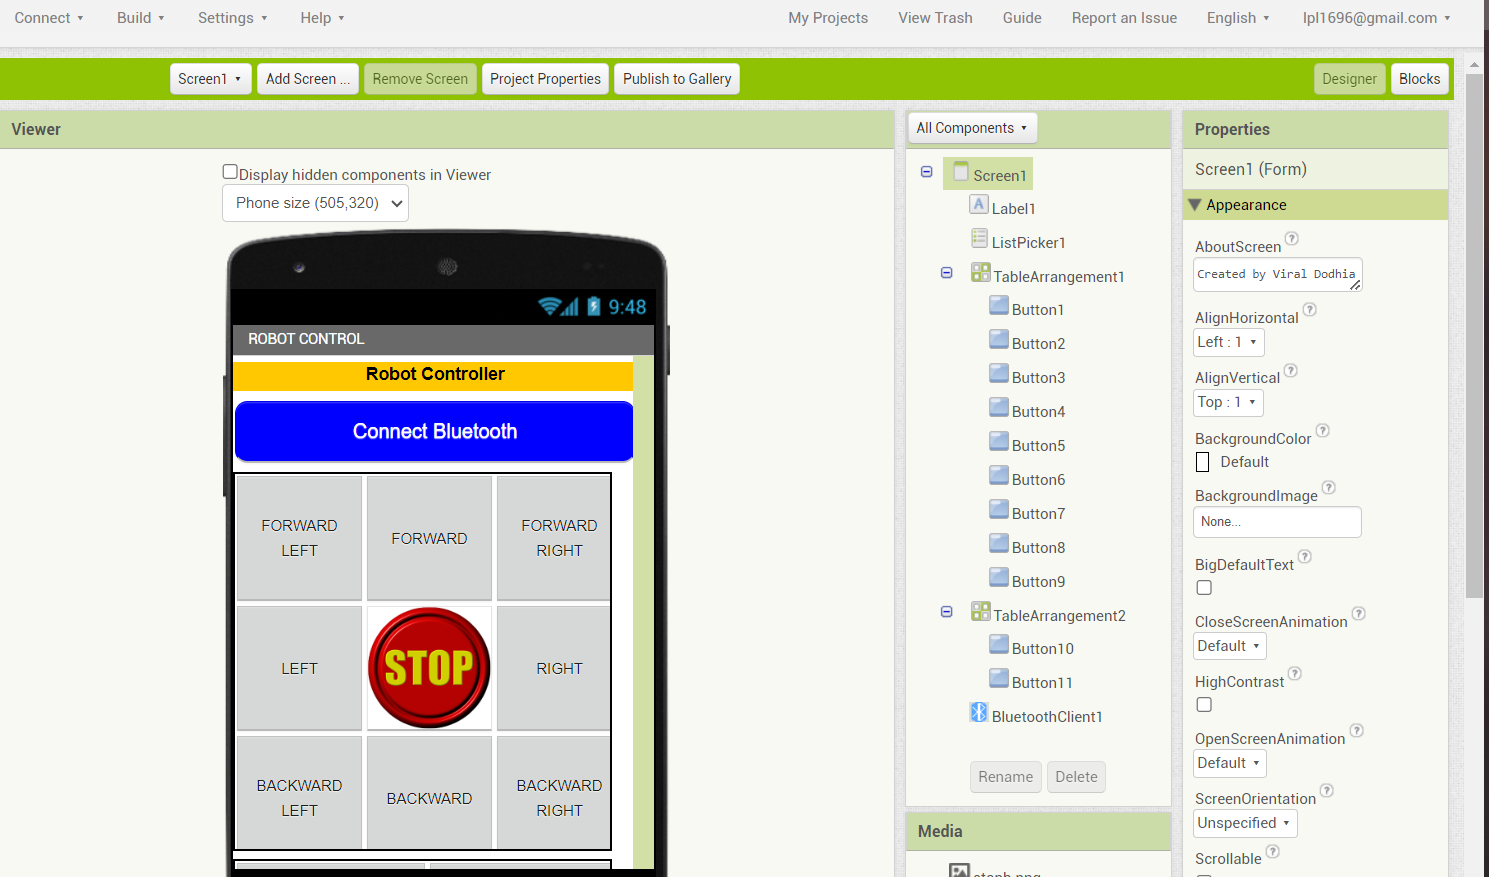
\includegraphics[width=0.5\textwidth]{figures/mit_app_inventor.png}
	\caption{Interface da plataforma MIT App Inventor}
	\label{fig:mit_app_inventor}
\end{figure}